\documentclass[draftmode,draftwater]{memarticle}
% \documentclass{memarticle}
\usepackage{paralist}
\usepackage[T1]{fontenc}
\usepackage{palatino%
           , pxfonts%
           , mathpazo%
}
\maxtocdepth{chapter}

% ------------------------------------------------------------

% Document title control. Change these as appropriate for your document.
% ------------------------------------------------------------
\newcommand{\doctitle}{CosmoSIS \\ Design and Plans}
\newcommand{\brieftitle}{CosmoSIS}
\newcommand{\authors}{\href{mailto:jbk@fnal.gov,paterno@fnal.gov}%
  {Jim Kowalkowski and Marc Paterno \\ \textit{Computing Division} \\
    \textit{SSI Group}}}

\newcommand{\docversion}{1}

% ------------------------------------------------------------
%  Define new commands here
% ------------------------------------------------------------
\newcommand{\prog}[1]% format to be used for program names
  {\texttt{#1}}
\newcommand{\facs}{\name{FACS}\xspace}
\newcommand{\cosmosis}{\name{CosmoSIS}\xspace}
\newcommand{\despipe}{\name{des-pipe}\xspace}


% ------------------------------------------------------------
%  Document starts here
% ------------------------------------------------------------
\listfiles
\begin{document}
	
\topmatter % include this to typeset the title, authors, and toc.

% ------------------------------------------------------------

\chapter{Details}

We propose the establishment of several source code repositories for
DES-developed analysis source code, with one repository for each
identified group of related codes. Use of a source code version control
system will allow DES scientists to share code more easily, and helps
assure reproducible results, because all ``production'' versions of DES
analysis modules will come from a known, and uniquely identifiable,
version of the DES source code.

\begin{fixme}
  For each section below, we should have the following issues covered:

  \begin{enumerate}
  \item Discussion
    \begin{itemize}
    \item Requirements
    \item Use cases
    \item Constraints
    \end{itemize}
  \item Possible directions
    \begin{itemize}
    \item Tools we use
    \item How it is now
    \item Where can it go?
    \end{itemize}
  \item Decisions
    \begin{itemize}
    \item What way should it go?
    \item What do users need to do as a result? How does existing code
      and practices need to change?
    \item What constraints/rules does it impose?
    \end{itemize}
  \end{enumerate}
\end{fixme}

\section{The \cosmosis framework}

We call the proposed framework \cosmosis. This is a framework
specifically for the creation of configurable sampling-based parameter
estimation programs. Each program consists of several different types of
components. These include:
\begin{itemize}
\item one \emph{sampler}, which is responsible for generating tuples in
  the parameter space according to some some sampling algorithm
  (possibly producing several tuples in parallel), and which invokes a
  \emph{likelihood function},
\item a \emph{likelihood function}, which is invoked by the sampler, to
  calculate the likelihood of the given parameter tuple; the likelihood
  function is composed from one or more \emph{physics modules},
\item a sequence of one or more \emph{physics modules} (see below).
\end{itemize}

The \emph{physics modules} are provided (though a standard interface)
the tuple of parameter values. Each physics module can read the values
of existing quantities, and calculate the values of derived quantities
(\eg spectra) that it can then add to the tuple. The physics modules are
run in a sequence determined by a configuration file, supplied by the
user, so that later physics modules can access the values of quantities
calculated by earlier physics modules. Each physics module also can (but
need not) contribute to the calculation of the likelihood of the
parameter vector. Figure~\ref{fig:despes} shows the organization of a
\cosmosis program.

\begin{figure}[htb]
  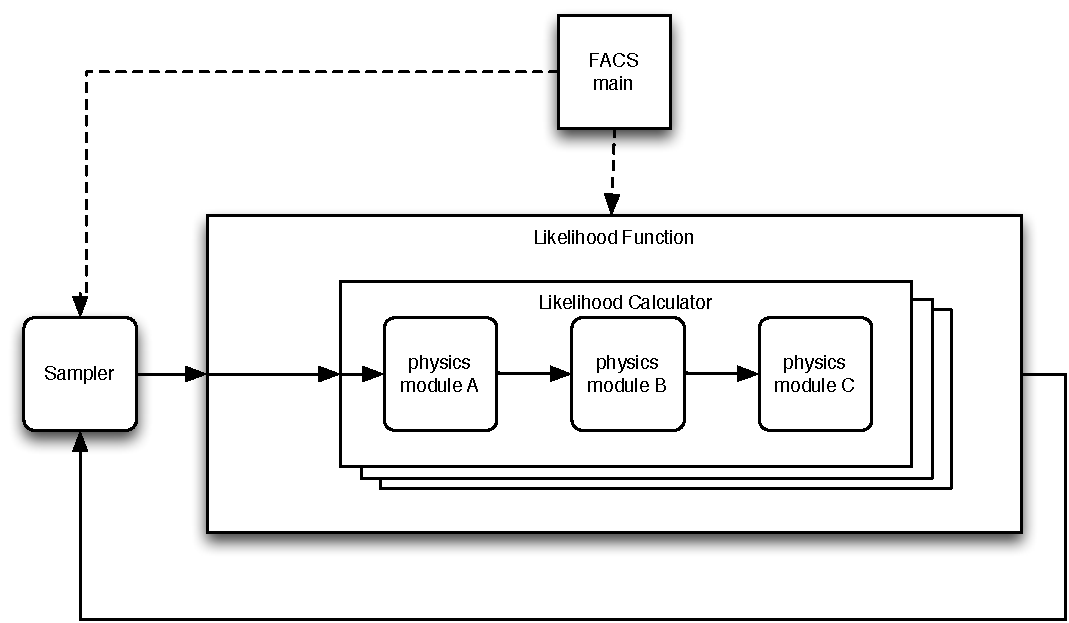
\includegraphics[width=\textwidth]{despes}
  \caption{The organization of a \cosmosis program. Solid arrows show
    the flow of parameter data. Dotted arrows show the flow of
    configuration data. Modules may also read ancillary data files, as
    directed by their configuration. The multiple likelihood calculator
    boxes indicate the possible parallel processing of multiple
    parameter vectors produced by the sampler.}
  \label{fig:despes}
\end{figure}

% \subsection{Discussion}
% blah.
% \subsubsection{Requirements}
% blah.
% \subsubsection{Use cases}
% blah.
% \subsubsection{Constraints}
% blah.

% \subsection{Possible directions}
% blah.
% \subsubsection{Tools we use}
% blah.
% \subsubsection{Existing situation}
% blah.
% \subsubsection{Options}
% blah.

% \subsubsection{Decisions}
% blah.
% \subsubsection{Suggested solution}
% blah.
% \subsubsection{Changes to existing code and practice}
% blah.
% \subsubsection{Resulting rules and conventions}
% blah.

\section{Physics modules}

Physics modules perform calculations of two types. They accept as input
a collection of model parameters, and can augment the collection with
derived quantities. They can not change the value of any
previously-calculated quantity. They can also calculate, and record, a
likelihood value, which will be combined with any other likelihoods
calculated by other modules in the program.

Physics modules are provided to the system by run-time configuration,
either through dynamically loaded libraries (for compiled languages) or
as Python modules.

Each physics module, at the time it is initialized, may be any data
files it needs to do its work. Typically, the names of the files to be
read will be supplied to the initialization code through the framework's
configuration mechanism.
% blah.
% \subsection{Discussion}
% blah.
% \subsubsection{Requirements}
% blah.
% \subsubsection{Use cases}
% blah.
% \subsubsection{Constraints}
% blah.

% \subsection{Possible directions}
% blah.
% \subsubsection{Tools we use}
% blah.
% \subsubsection{Existing situation}
% blah.
% \subsubsection{Options}
% blah.

% \subsubsection{Decisions}
% blah.
% \subsubsection{Suggested solution}
% blah.
% \subsubsection{Changes to existing code and practice}
% blah.
% \subsubsection{Resulting rules and conventions}
% blah.


\subsection{Samplers}


\subsection{Physics calculators}

\subsection{Likelihood calculators}

\section{Configuration}

% \subsection{Discussion}
% blah.
% \subsubsection{Requirements}
% blah.
% \subsubsection{Use cases}
% blah.
% \subsubsection{Constraints}
% blah.

% \subsection{Possible directions}
% blah.
% \subsubsection{Tools we use}
% blah.
% \subsubsection{Existing situation}
% blah.
% \subsubsection{Options}
% blah.

% \subsubsection{Decisions}
% blah.
% \subsubsection{Suggested solution}
% blah.
% \subsubsection{Changes to existing code and practice}
% blah.
% \subsubsection{Resulting rules and conventions}
% blah.


\subsection{Whole program configuration}


\subsection{Module configuration}


\section{Packaging}


% \subsection{Discussion}
% blah.
% \subsubsection{Requirements}
% blah.
% \subsubsection{Use cases}
% blah.
% \subsubsection{Constraints}
% blah.

% \subsection{Possible directions}
% blah.
% \subsubsection{Tools we use}
% blah.
% \subsubsection{Existing situation}
% blah.
% \subsubsection{Options}
% blah.

% \subsubsection{Decisions}
% blah.
% \subsubsection{Suggested solution}
% blah.
% \subsubsection{Changes to existing code and practice}
% blah.
% \subsubsection{Resulting rules and conventions}
% blah.

\section{Provenance and storage}


% \subsection{Discussion}
% blah.
% \subsubsection{Requirements}
% blah.
% \subsubsection{Use cases}
% blah.
% \subsubsection{Constraints}
% blah.

% \subsection{Possible directions}
% blah.
% \subsubsection{Tools we use}
% blah.
% \subsubsection{Existing situation}
% blah.
% \subsubsection{Options}
% blah.

% \subsubsection{Decisions}
% blah.
% \subsubsection{Suggested solution}
% blah.
% \subsubsection{Changes to existing code and practice}
% blah.
% \subsubsection{Resulting rules and conventions}
% blah.


\section{Development environment and strategy}


% \subsection{Discussion}
% blah.
% \subsubsection{Requirements}
% blah.
% \subsubsection{Use cases}
% blah.
% \subsubsection{Constraints}
% blah.

% \subsection{Possible directions}
% blah.
% \subsubsection{Tools we use}
% blah.
% \subsubsection{Existing situation}
% blah.
% \subsubsection{Options}
% blah.

% \subsubsection{Decisions}
% blah.
% \subsubsection{Suggested solution}
% blah.
% \subsubsection{Changes to existing code and practice}
% blah.
% \subsubsection{Resulting rules and conventions}
% blah.

\chapter{Moving forward}

Priority, plans.

\chapter{Relationship to other work}

\begin{itemize}
\item Salman's project?
\item LSST DESC?
\end{itemize}

\bibliographystyle{ieeetr}
\bibliography{cosmosis}


\end{document}

%%% Local Variables:
%%% mode: latex
%%% TeX-master: t
%%% End:
